Siden NPN-transistoren består av 2 PN-overganger,
kan man anse det som to dioder koblet sammen.
\\\\
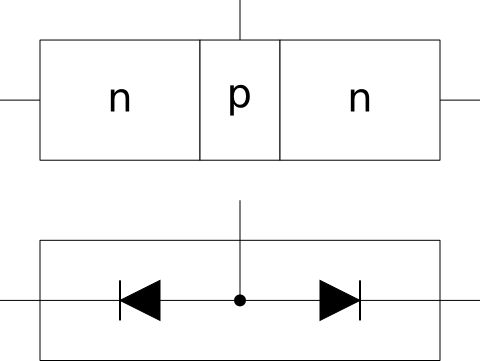
\includegraphics[width=0.5\textwidth]{./img/npn-bias}
\\\\
Disse diodene kan kjøres i forskjellig bias (forward, reverse).
Avhengig av forholdet mellom spenningen
ved diodens collector, base og emitter, fungerer transistoren forskjellig.

De forskjellige kombinasjonene utgjør transistorens operasjonsmodi.
\\\\
\begin{tabular}{ l | c | r}
Base-Emitter & Base-Collector & Operasjonsmodi \\ \hline
Reverse & Reverse & Cutoff \\
Forward & Reverse & Aktiv \\
Forward & Forward & Metning \\
\end{tabular}
